The multi--jet background events are mainly due to mis--reconstruction or loss
in some dead part of the calorimeter of jets or to the presence of neutrinos in
some heavy--flavor hadronic decay. The acceptance in the SR for multi--jet
events is low, nevertheless the large cross section of this process could
potentially lead to a high contamination in the SR\@. The use of MC simulation
in order to estimate the contribution to BG of this process is very difficult
due to the very large MC samples that would be required and the detailed
modeling of any calorimeter defects. For these reasons a data--driven technique,
the \emph{jet smearing method}, is used. It addresses event topologies with
large $\met$ originating from jet mis-reconstruction. This method creates large
sample of well measured low $\met$ jets called \emph{seeds} which are
\emph{smeared} using a function that quantify the $\pt$ fluctuation of a
measured reconstructed jet (the \emph{response function}) to create $\met$ in
the event. This process is reiterated many times to create a \emph{pseudo-data}
sample that is used in the SR analysis selection to estimate the distribution of
variables defining the control and signal regions. The procedure is described in
more details in Ref.~\cite{JetSmearing}. The multi-jet control region is defined
by inverting the $\Delta \phi_\mathrm{\, min} (\met, \mathrm{jet})$ and applying
the inclusive and exclusive SR $\met$ cuts. For the EM1 and IM1 the multi-jet
background constitutes the 0.5\% of the total BG and it is negligible in other
signal regions.
% \begin{figure}[!h]
%   \centering
%   \begin{subfigure}[t]{.48\linewidth}
%     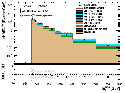
\includegraphics[width=\linewidth]{multijet_et_miss}
%     \caption{$\met$ distribution.}
%     \label{fig:dimuon_cr_et_miss_pre_fit}
%   \end{subfigure}
%   \begin{subfigure}[t]{.48\linewidth}
%     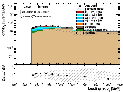
\includegraphics[width=\linewidth]{multijet_jet1_pt}
%     \caption{Leading jet $\pt$ distribution.}
%     \label{fig:dimuon_cr_jet1_pt_pre_fit}
%   \end{subfigure}
%   \caption{The $\met$ and the leading jet $\pt$ key variable distribution in the
%     multi-jet control region with $\pt > 250$~GeV and $\met > 250$~GeV.}
%   \label{fig:multijet_distributions}
% \end{figure}
%%% Local Variables:
%%% mode: latex
%%% TeX-master: "../search_for_DM_LED_with_ATLAS"
%%% End:
